\documentclass[a4paper]{article}

% Expanded on 2022-03-28 at 10:16:21.

\usepackage{../../style}

\title{Analyse 2}
\author{Joachim Favre}
\date{Lundi 28 mars 2022}

\begin{document}
\maketitle

\lecture{11}{2022-03-28}{Et le retour des différences maintenant! \smiley}{
\begin{itemize}[left=0pt]
    \item Définition des dérivées partielles.
    \item Définition du gradient.
    \item Définition des dérivées directionnelles.
    \item Définition de la dérivabilité.
\end{itemize}

}

\section[Calcul différentiel]{Calcul différentiel des fonctions de plusieurs variables}
\subsection{Dérivée partielles et le gradient}
\parag{Définition: dérivée partielle}{
    Soit $f: E \mapsto \mathbb{R}^n$ une fonction, où $E \subset \mathbb{R}^n$ est un ensemble ouvert, et soit la fonction d'une seule variable suivante: 
    \[g\left(s\right) = f\left(a_1, a_2, \ldots, a_{k-1}, s, a_{k+1}, \ldots, a_n\right), \mathspace \text{où } \bvec{a} = \left(a_1, \ldots, a_n\right) \in E\]
    
    Le domaine de définition de $g$ est:
    \[D_g = \left\{s \in \mathbb{R} \telque \left(a_1, a_2, \ldots, a_k, s, a_{k+1}, \ldots, a_n\right) \in E\right\}\]
     
    Alors, si $g$ est dérivable en $a_k \in D_g$, on dit que la \important{$k$-ème dérivée partielle} de $f$ en $\bvec{a} \in E$ existe est égale à $g'\left(a_k\right)$, notée: 
    \[g'\left(a_k\right) \over{=}{déf} \frac{\partial f}{\partial x_k}\left(\bvec{a}\right) = D_k f\left(\bvec{a}\right)\]
    
    On remarque que nous avons: 
    \[\frac{\partial f}{\partial x_k}\left(\bvec{a}\right) = \lim_{t \to 0} \frac{g\left(a_k + t\right) - g\left(a_k\right)}{t} = \lim_{t \to 0} \frac{f\left(\bvec{a} + t \bvec{e_k}\right) - f\left(\bvec{a}\right)}{t}\]
    
    \subparag{Remarque}{
        Quand on prend une dérivée partielle, on considère que tout est constant, sauf la variable selon laquelle nous calculons notre dérivée.
    }
}

\parag{Exemple}{
    Soit la fonction $f\left(x, y\right) = \sin\left(xy\right)$ où $f: \mathbb{R}^2 \mapsto \mathbb{R}$. Soit aussi $\left(x_0, y_0\right) \in \mathbb{R}^2$. Nous voulons calculer la dérivée partielle selon $x$ en $\left(x_0, y_0\right)$:
    \[\frac{\partial f}{\partial x}\left(x_0, y_0\right) = \lim_{t \to 0} \frac{f\left(x_0 + t, y_0\right) - f\left(x_0, y_0\right)}{t} = \lim_{t \to 0} \frac{\sin\left(\left(x_0 + t\right)y_0\right) - \sin\left(x_0 y_0\right)}{t}\]
    
    Si $y_0 = 0$, alors nous avons: 
    \[\frac{\partial f}{\partial x}\left(x_0, 0\right) = \lim_{t \to 0} \frac{\sin\left(0\right) - \sin\left(0\right)}{t} = 0\]
    
    Si $y_0 \neq 0$: 
    \begin{multiequality}
    \frac{\partial f}{\partial x}\left(x_0, y_0\right) =\ & \lim_{t \to 0} \frac{\sin\left(x_0 y_0\right)\cos\left(t y_0\right) + \cos\left(x_0 y_0\right) \sin\left(ty_0\right) - \sin\left(x_0 y_0\right)}{t} \\
    =\ & \lim_{t \to 0} \left(y_0 \sin\left(x_0 y_0\right) \cdot \underbrace{\frac{\cos\left(t y_0\right) - 1}{t y_0}}_{\to 1} + y_0 \cos\left(x_0 y_0\right) \underbrace{\frac{\sin\left(t y_0\right)}{t y_0}}_{\to 1}\right)  \\
    =\ & y_0 \cos\left(x_0 y_0\right)
    \end{multiequality}
    
    On obtient donc: 
    \[\frac{\partial }{\partial x}\sin\left(x, y\right) \eval_{\left(x_0, y_0\right)}^{} = y_0 \cos\left(x_0, y_0\right)\]
        
    Nous avons calculé cette dérivée par la définition, cependant, nous pouvons aller beaucoup plus rapidement en utilisant notre remarque ci-dessus (quand on prend une dérivée partielle selon $y$, on considère $x$ comme constant): 
    \[\frac{\partial f}{\partial y}\left(x_0, y_0\right) = x_0 \cos\left(x_0, y_0\right)\]
}

\parag{Définition: Gradient}{
    Si toutes les dérivées partielles existent en $\bvec{a} \in E$: 
    \[\frac{\partial f}{\partial x_1}\left(\bvec{a}\right), \mathspace \ldots, \mathspace \frac{\partial f}{\partial x_n}\left(\bvec{a}\right)\]
    
    Alors, on définit le \important{gradient} de $f$ en $\bvec{a}$ comme: 
    \[\nabla f\left(\bvec{a}\right) = \left(\frac{\partial f}{\partial x_1}\left(\bvec{a}\right), \ldots, \frac{\partial f}{\partial x_n}\left(\bvec{a}\right)\right)\]
    
    Notez que $\nabla$ s'appelle le \important{nabla}, et ce symbole se révélera très utile par la suite.

    \subparag{Intuition}{
        Le gradient montre la direction de la plus grande pente de la fonction. En d'autres mots, si la fonction représente une altitude en fonction d'une position, alors le gradient montre dans quelle direction nous devrons aller pour monter le plus vite. Nous prenons cette propriété telle quelle pour l'instant, mais nous la démontrons dans le cours suivant.
    }
}

\parag{Exemple 1}{
    Reprenons notre fonction $f\left(x, y\right) = \sin\left(xy\right)$. Nous avions déjà calculé les dérivées partielles, donc: 
    \[\nabla f\left(x, y\right) = \left(y \cos\left(xy\right), x\cos\left(xy\right)\right), \mathspace \forall \left(x, y\right) \in \mathbb{R}^2\]
    
    Voici le graphique de notre fonction: 
    \begin{center}
    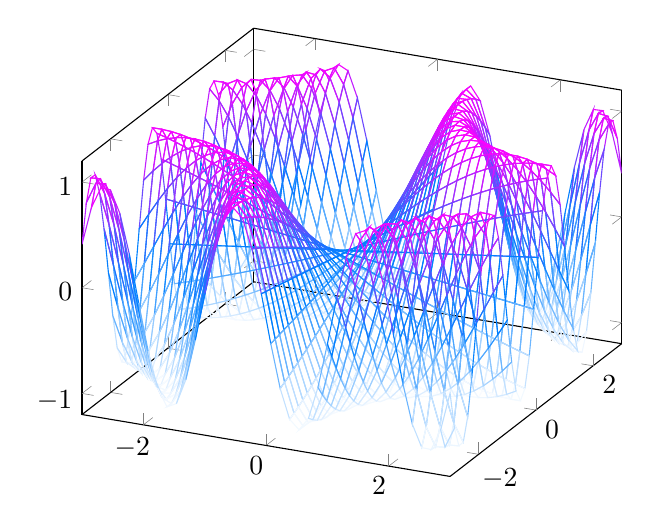
\begin{tikzpicture}
        \begin{axis}[
            %view={-45}{45}
        ]
        \addplot3[
            mesh,
            samples=40,
            domain=-3:3,
            colormap/cool,
        ]
        {sin(x*y * 180/pi)};
        \end{axis}
    \end{tikzpicture}
    \end{center}

    Nous pouvons visualiser le \important{champ vectoriel} du gradient, c'est-à-dire:
    \[\begin{split}
    \nabla f: \mathbb{R}^2 &\longmapsto \mathbb{R}^2 \\
    \left(x, y\right) &\longmapsto \nabla f\left(\left(x, y\right)\right)
    \end{split}\]
    
    \begin{center}
    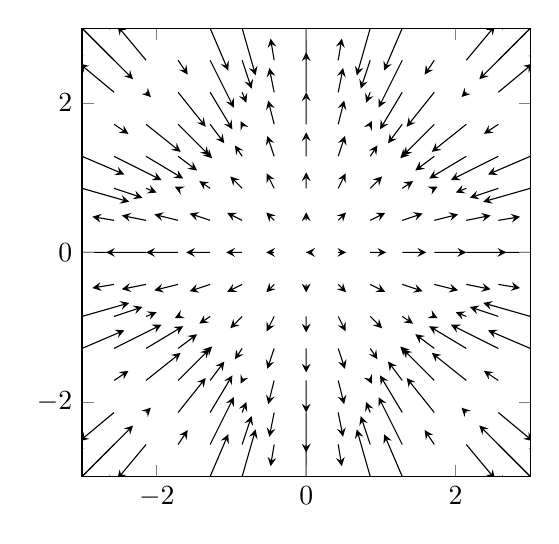
\begin{tikzpicture}
    \begin{axis}[
    xmin = -3, xmax = 3,
    ymin = -3, ymax = 3,
    zmin = 0, zmax = 1,
    axis equal image,
    view = {0}{90},
    ]
    \addplot3[
        quiver = {
            u = {x*cos(x*y * 180/pi)},
            v = {y*cos(x*y * 180/pi)},
            scale arrows = 0.25,},
        -stealth,
        domain = -3:3,
        domain y = -3:3,
        samples=15,
    ] {0};
    \end{axis}
    \end{tikzpicture}
    \end{center}
}

\parag{Exemple 2}{
    Soit la fonction $f\left(x, y\right) = x^2 + y^2$, où $f: \mathbb{R}^2 \mapsto \mathbb{R}^2$. Alors: 
    \[\nabla f\left(x, y\right) = \left(2x, 2y\right), \mathspace \forall \left(x, y\right) \in \mathbb{R}^2\]
    
    Nous pouvons dessiner le graphique de la fonction et le champ de vecteurs de son gradient:
    \begin{center}
    \begin{minipage}{0.49\textwidth}
    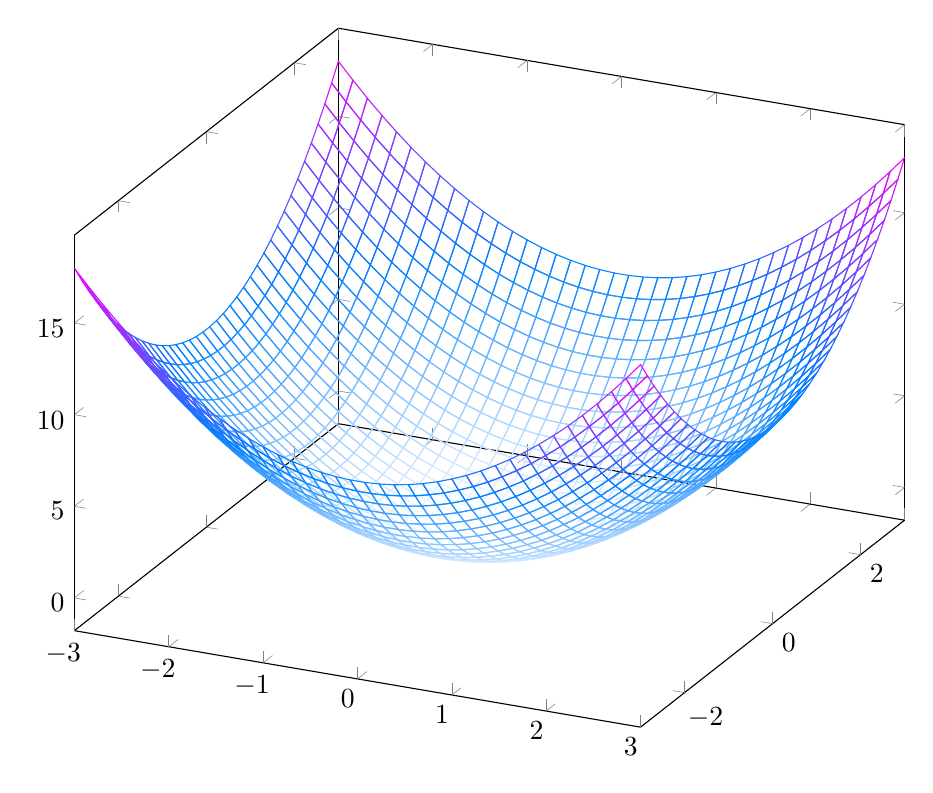
\begin{tikzpicture}
        \begin{axis}[
            width=\textwidth,
            %view={-45}{45}
        ]
        \addplot3[
            mesh,
            samples=40,
            domain=-3:3,
            colormap/cool,
        ]
        {x*x + y*y};
        \end{axis}
    \end{tikzpicture}
    \end{minipage}
    \begin{minipage}{0.49\textwidth}
    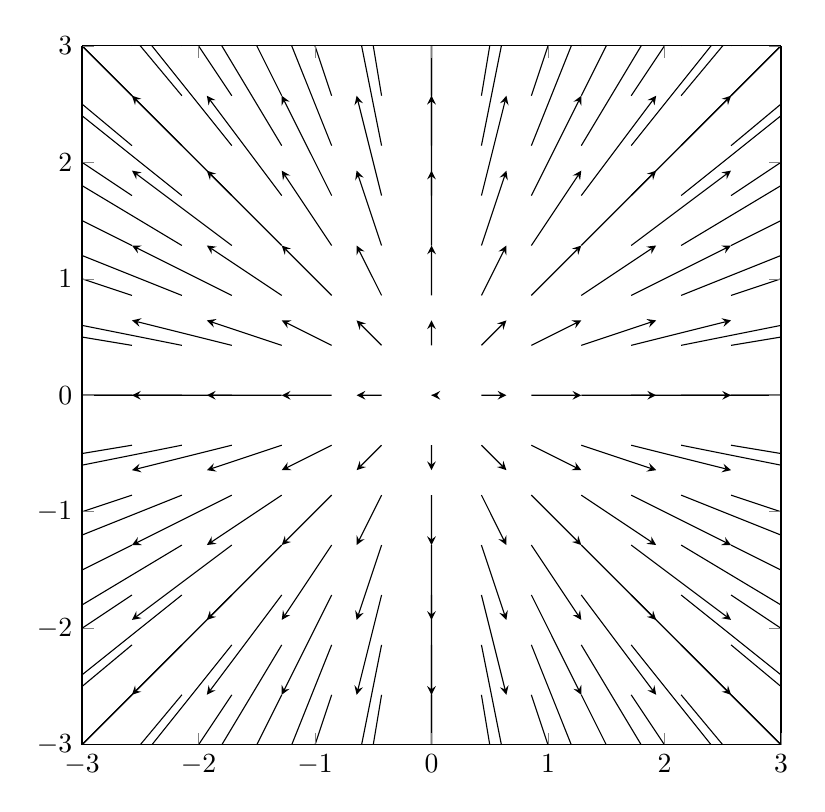
\begin{tikzpicture}
    \begin{axis}[
        width=\textwidth,
        xmin = -3, xmax = 3,
        ymin = -3, ymax = 3,
        zmin = 0, zmax = 1,
        axis equal image,
        view = {0}{90},
    ]
    \addplot3[
        quiver = {
            u = {2*x},
            v = {2*y},
            scale arrows = 0.25,},
        -stealth,
        domain = -3:3,
        domain y = -3:3,
        samples=15,
    ] {0};
    \end{axis}
    \end{tikzpicture}
    \end{minipage}
    \end{center}

    Nous pouvons aussi calculer une dérivée partielle par la définition:
    \[\frac{\partial f}{\partial x}\left(x_0, y_0\right) = \lim_{t \to 0} \frac{\left(x_0 + t\right)^2 + y_0^2 - x_0^2 - y_0^2}{t} = \lim_{t \to 0} \frac{x_0^2 + 2x_0t + t^2 - x_0^2}{t} = 2x_0\]
}

\parag{Définition: Dérivée directionnelle}{
    Soit $E \subset \mathbb{R}^n$ un sous-ensemble ouvert. Soient aussi $\bvec{a} \in E$, et $\bvec{v} \in\mathbb{R}^n$ où $\bvec{v} \neq \bvec{0}$.

    Nous savons que la droite passant par $\bvec{a}$ en direction de $\bvec{v}$ admet la paramétrisation suivante: 
    \[\bvec{\ell}\left(t\right) = \bvec{a} + t \bvec{v}, \mathspace \forall t \in \mathbb{R}\]

    \imagehere[0.5]{DeriveeDirectionnelle.png}
    
    Considérons une fonction $f :E \mapsto \mathbb{R}$, et soit la fonction d'une variable $t$ suivante:
    \[g\left(t\right) \over{=}{déf} f\left(\bvec{\ell}\left(t\right)\right) = f\left(\bvec{a} + t \bvec{v}\right), \mathspace \forall t \in \left\{t \in \mathbb{R} \telque \bvec{a} + t \bvec{v} \in E\right\}\]

    Si $g$ est dérivable en $t = 0$, on dit qu'il existe la \important{dérivée directionnelle} de $f$ en $\bvec{a}$ suivant le vecteur $\bvec{v}$ (dans la direction de $\bvec{v}$). La dérivée directionnelle de $f$ en $\bvec{a}$ en direction de $\bvec{v}$ est donnée par: 
    \[\lim_{t \to 0} \frac{g\left(t\right) - g\left(0\right)}{t} = \lim_{t \to 0} \frac{f\left(\bvec{a} + t \bvec{v}\right) - f\left(\bvec{a}\right)}{t} \over{=}{déf}  Df\left(\bvec{a}, \bvec{v}\right) = \frac{\partial f}{\partial \bvec{v}}\left(\bvec{a}\right)\]

    \subparag{Remarque}{
        \begin{enumerate}[left=0pt]
            \item Si $\bvec{v} = \bvec{e_i}$, où $\bvec{e_i} = \left(0, \ldots, 0, 1, 0, \ldots, 0\right)$, alors: 
                \[Df\left(\bvec{a}, \bvec{e_i}\right) = \lim_{t \to 0} \frac{f\left(\bvec{a} + t \bvec{e_i}\right) - f\left(\bvec{a}\right)}{t} = \frac{\partial f}{\partial x_i}\left(\bvec{a}\right)\]
            
                En d'autres mots, la dérivée partielle est un cas particulier de la dérivée directionnelle.

                Ainsi, si toutes les dérivées directionnelles existent en $\bvec{a}$ (pour tout $\bvec{v} \neq \bvec{0}$), alors toutes les dérivées partielles existent aussi en ce point. Cependant, la réciproque est fausse en générale.
            \item Essayons de multiplier $\bvec{v}$ par $\lambda \in \mathbb{R}^*$:
                \begin{multiequality}
                D f\left(\bvec{a}, \lambda \bvec{v}\right) & = \lim_{t \to 0} \frac{f\left(\bvec{a} + t \lambda \bvec{v}\right) - f\left(\bvec{a}\right)}{t}  \\
                 & \over{=}{$s = t\cdot \lambda$} \lim_{s \to 0} \frac{f\left(\bvec{a} + s \bvec{v}\right) - f\left(\bvec{a}\right)}{\frac{s}{\lambda}}  \\
                & = \lim_{s \to 0} \frac{f\left(\bvec{a}+ s \bvec{v}\right) - f\left(\bvec{a}\right)}{s} \lambda  \\
                & = Df\left(\bvec{a}, \bvec{v}\right) \lambda 
                \end{multiequality}

                C'est cohérent car ce qui nous importe est la direction est non pas la longueur de notre vecteur. 

                Donc, si la dérivée directionnelle de $f$ en $\bvec{a}$ suivant $\bvec{v}$ existe, alors la dérivée directionnelle de $f$ en $\bvec{a}$ suivant $\lambda \bvec{v}$ existe pour tout $\lambda \in \mathbb{R}^*$. Il suffit donc de calculer les dérivées directionnelles suivant les vecteurs unitaires $\left\|\bvec{v}\right\| = 1$.
        \end{enumerate}
        
    }
}

\parag{Exemple}{
    Prenons la fonction suivante: 
    \[f\left(x, y\right) = x^2 + y^2\]
    
    Nous voulons calculer $Df\left(\bvec{a}, \bvec{v}\right)$, où $\bvec{a} = \left(1, 1\right)$ et $\bvec{v} = \left(\frac{1}{2}, \frac{\sqrt{3}}{2}\right)$: 
    \[D f\left(\bvec{a}, \bvec{v}\right) = \lim_{t \to 0} \frac{f\left(\bvec{a} + t \bvec{v}\right) - f\left(\bvec{a}\right)}{t} = \lim_{t \to 0} \frac{\left(1 + \frac{1}{2} t\right)^2 + \left(1 + \frac{\sqrt{3}}{2}\right)^2 - 1^2 - 1^2}{t} \]

    Ce qui est égal à: 
    \[\lim_{t \to 0} \frac{1 + t + \frac{1}{4} t^2 + 1 + \sqrt{3}t + \frac{3}{4}t^2 - 1 - 1}{t} = \lim_{t \to 0} \frac{t + \sqrt{3}t + t^2}{t} = 1 + \sqrt{3}\]
    
    
    Nous allons voir bientôt une méthode de calcul plus rapide.
}

\subsection{Dérivabilité et différentielle}
\parag{Définition: dérivabilité}{
    Soit $f: E \mapsto \mathbb{R}$, où $E \subset \mathbb{R}^n$ est ouvert. De plus, soit $\bvec{a} \in E$.

    On dit que $f$ est \important{dérivable} (ou \important{différentiable}) au point $\bvec{a}$ s'il existe une transformation linéaire $L_{\bvec{a}} : \mathbb{R}^n \mapsto \mathbb{R}$ et une fonction $r: E \mapsto \mathbb{R}$ telles que: 
    \[f\left(\bvec{x}\right) = f\left(\bvec{a}\right) + L_{\bvec{a}}\left(\bvec{x} - \bvec{a}\right) + r\left(\bvec{x}\right), \mathspace\forall x \in E\]
    et aussi $r$ doit être telle que: 
    \[\lim_{\bvec{x} \to \bvec{a}} \frac{r\left(\bvec{x}\right)}{\left\|\bvec{x} - \bvec{a}\right\|} = 0\]
    
    $L_{\bvec{a}}$ s'appelle la \important{différentielle} de $f$ au point $\bvec{a} \in E$, et est aussi parfois notée: 
    \[L_{\bvec{a}} = df\left(\bvec{a}\right)\]

    \subparag{Intuition}{
        Cette définition veut dire que notre fonction admet une linéarisation: elle se comporte comme un hyperplan autour d'un point.
    }
    
    \subparag{Transformation linéaire}{
        Une transformation linéaire $T : \mathbb{R}^n \mapsto \mathbb{R}$ est une fonction telle que: 
        \[T\left(\alpha \bvec{x} + \beta \bvec{y}\right) = \alpha T\left(\bvec{x}\right) + \beta T\left(\bvec{y}\right), \mathspace \forall \bvec{x}, \bvec{y} \in \mathbb{R}^n, \forall \alpha, \beta \in \mathbb{R}\]
         
        En particulier, cela nous donne: 
        \[T\left(\bvec{0}\right) = \bvec{0}\]
        
        Par exemple, $T\left(x, y\right) = x + y$ est une application linéaire $\mathbb{R}^2 \mapsto \mathbb{R}$, mais $T\left(x, y\right) = x + y + 2$ n'est pas une application linéaire (même si c'est une fonction linéaire, puisque c'est un polynôme).
    }

    \subparag{Remarque}{
        Comparons notre définition avec la dérivabilité des fonctions d'une seule variable. 

        Une fonction $f: I \mapsto \mathbb{R}$, où $I \subset \mathbb{R}$ est un sous-ensemble ouvert, est différentiable en $a \in I$ s'il existe $\ell \in \mathbb{R}$ et une fonction $r: I \mapsto \mathbb{R}$ tels que: 
        \[f\left(x\right) = f\left(a\right) + \ell\left(x - a\right) + r\left(x\right), \ \forall x \in I, \text{ et } \lim_{x \to a} \frac{r\left(x\right)}{\left|x - a\right|} = 0\]
        
        Or, une constante $L\left(x\right) = \ell x$ est une application linéaire $\mathbb{R}^{1} \mapsto \mathbb{R}^1$ (un scalaire est comme une matrice de dimension $1 \times 1$). De plus, dans ce cas, nous avions $\ell = f'\left(a\right)$, cela semble donc cohérent avec le fait que $L_{\bvec{a}} = df\left(\bvec{a}\right)$ est appelée la différentielle.

        En d'autres mots, notre définition de dérivabilité s'applique dans le cas $n = 1$. 
    }

}





\end{document}
